%
% morse.tex
%
% (c) 2021 Prof Dr Andreas Müller, OST Ostschweizer Fachhochschule
%
\documentclass[tikz]{standalone}
\usepackage{times}
\usepackage{amsmath}
\usepackage{txfonts}
\usepackage[utf8]{inputenc}
\usepackage{graphics}
\usetikzlibrary{arrows,intersections,math}
\usepackage{ifthen}
\begin{document}

\newboolean{showgrid}
\setboolean{showgrid}{false}
\def\breite{7}
\def\hoehe{4}

\begin{tikzpicture}[>=latex,thick]

% Povray Bild
\begin{scope}[xshift=-3.3cm]
\node at (0,0) {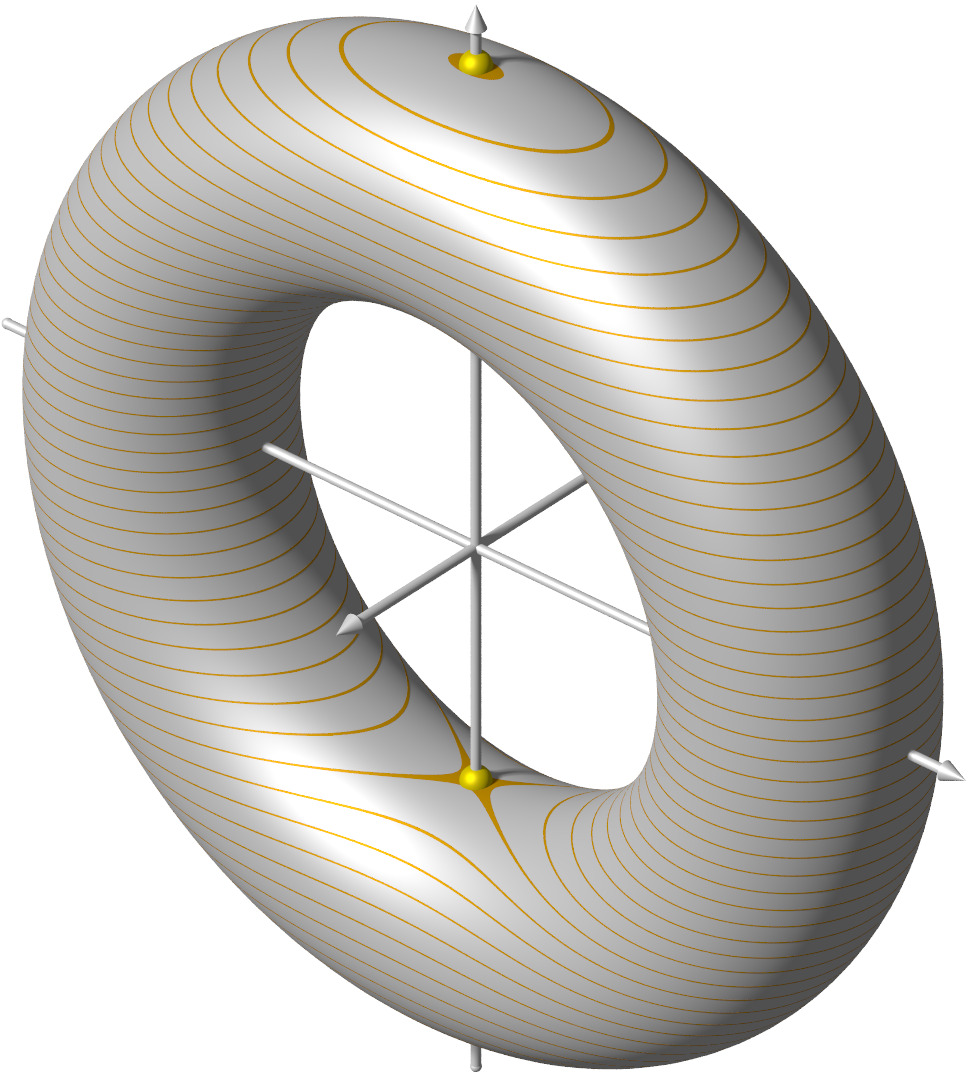
\includegraphics[width=6cm]{torus-levels.jpg}};
\end{scope}
\begin{scope}[xshift=3.3cm]
\node at (0,0) {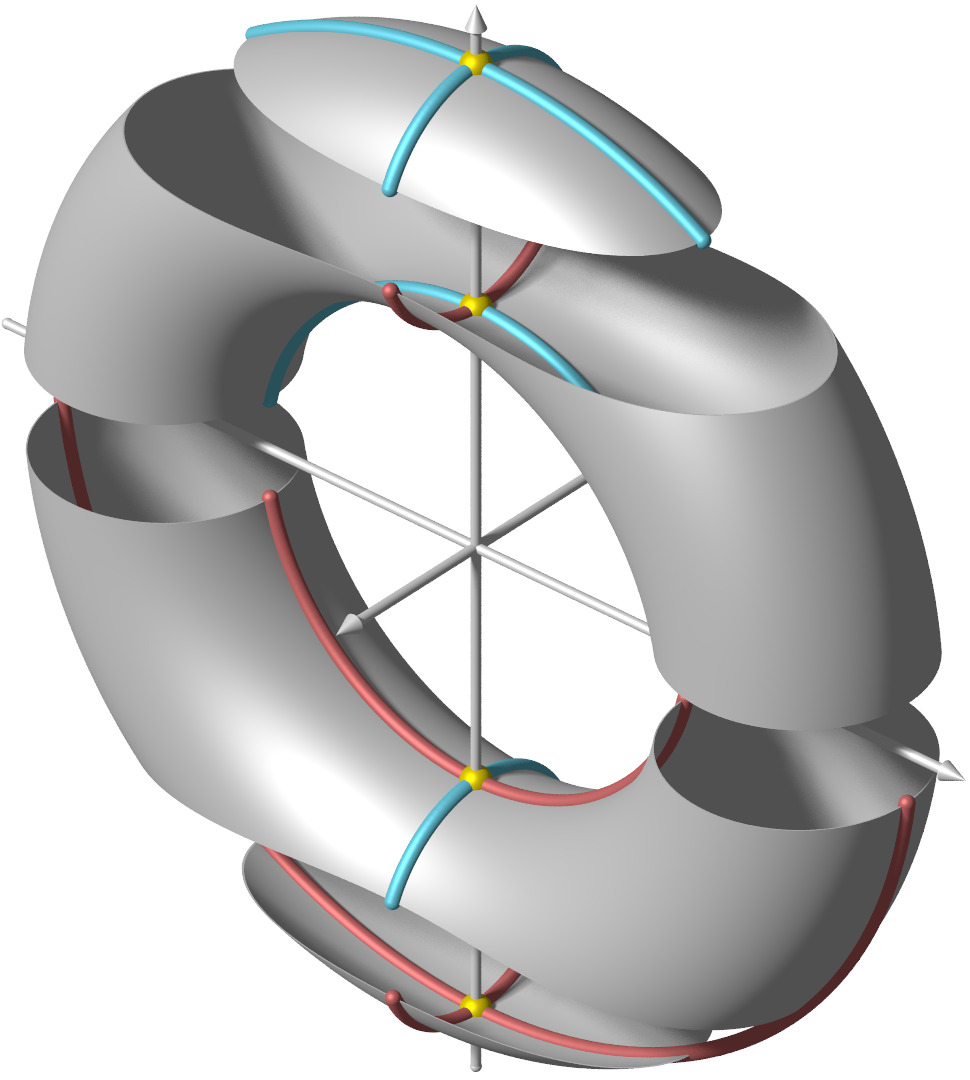
\includegraphics[width=6cm]{torus-morse.jpg}};
\end{scope}

% Gitter
\ifthenelse{\boolean{showgrid}}{
\draw[step=0.1,line width=0.1pt] (-\breite,-\hoehe) grid (\breite, \hoehe);
\draw[step=0.5,line width=0.4pt] (-\breite,-\hoehe) grid (\breite, \hoehe);
\draw                            (-\breite,-\hoehe) grid (\breite, \hoehe);
\fill (0,0) circle[radius=0.05];
}{}

\node at (3.7,3) [right] {Index 2};
\node at (3.4,1.45) [right] {Index 1};
\node at (3.1,-1.5) [left] {Index 1};
\node at (2.7,-2.9) [left] {Index 0};

\end{tikzpicture}

\end{document}

